\subsection{Número promedio de viajes}

Los datos abiertos de MiBici contienen un identificador de usuario, por lo que se puede saber el número de viajes realizados en un día por todos los usuarios.

\subsubsection{Promedio mensual por hora}

Se procedió a obtener un promedio mensual del número de viajes realizados por hora. El promedio mensual por hora se realizo usando la ecuación \ref{eq:monthly_hourly_mean_count_travel}.

\begin{equation}
    \bar{V}_{m,h} = \frac{1}{n_{(m,h)}} \sum_{i=1}^{n_{(m,n)}} \hat{V}_{i} \qquad \begin{matrix}
        m=1,2,\dots,12 \\ h=6,7,\dots,23
    \end{matrix} \label{eq:monthly_hourly_mean_count_travel}
\end{equation}

donde $\hat{V}$ y $n_{(m,n)}$ es el conjunto y la cantidad total de viajes realizados para el mes $m$ realizados entre las $h$ y $h+1$ horas respectivamente. De una manera semejante, se calculo la varianza de este conjunto con la ecuación \ref{eq:monthly_hourly_var_count_travel}.

\begin{equation}
    \sigma_{V_{(m,h)}} = \frac{1}{n_{(m,h)}-1} \sum_{i=1}^{n_{(m,n)}} (V_i-\bar{V}_{(m,h)})^2 \qquad \begin{matrix}
        m=1,2,\dots,12 \\ h=6,7,\dots,23
    \end{matrix} \label{eq:monthly_hourly_var_count_travel}
\end{equation}

En la figura \ref{fig:monthly_hourly_count_travel} se muestran los resultados de aplicar las ecuaciones \ref{eq:monthly_hourly_mean_count_travel} y \ref{eq:monthly_hourly_var_count_travel} a el número de viajes.

En la figura \ref{fig:monthly_hourly_count_travel} se visualiza que existe un aumento en el número de viajes entre los meses septiembre y diciembre. Lo cual coincide con lo antes planteado con las figuras \ref{fig:monthly_hourly_distance} y \ref{fig:monthly_hourly_time}. En la figura \ref{fig:monthly_hourly_var_count_travel} se observa como el número de usuarios tiene una variación mayor a las 8, y 18 horas. Esto puede deberse a la elección de los usuarios por que servicio de transporte público les hes mejor tomar en un día.

\begin{figure}[H]
    \centering
    \begin{subfigure}[b]{8cm}
        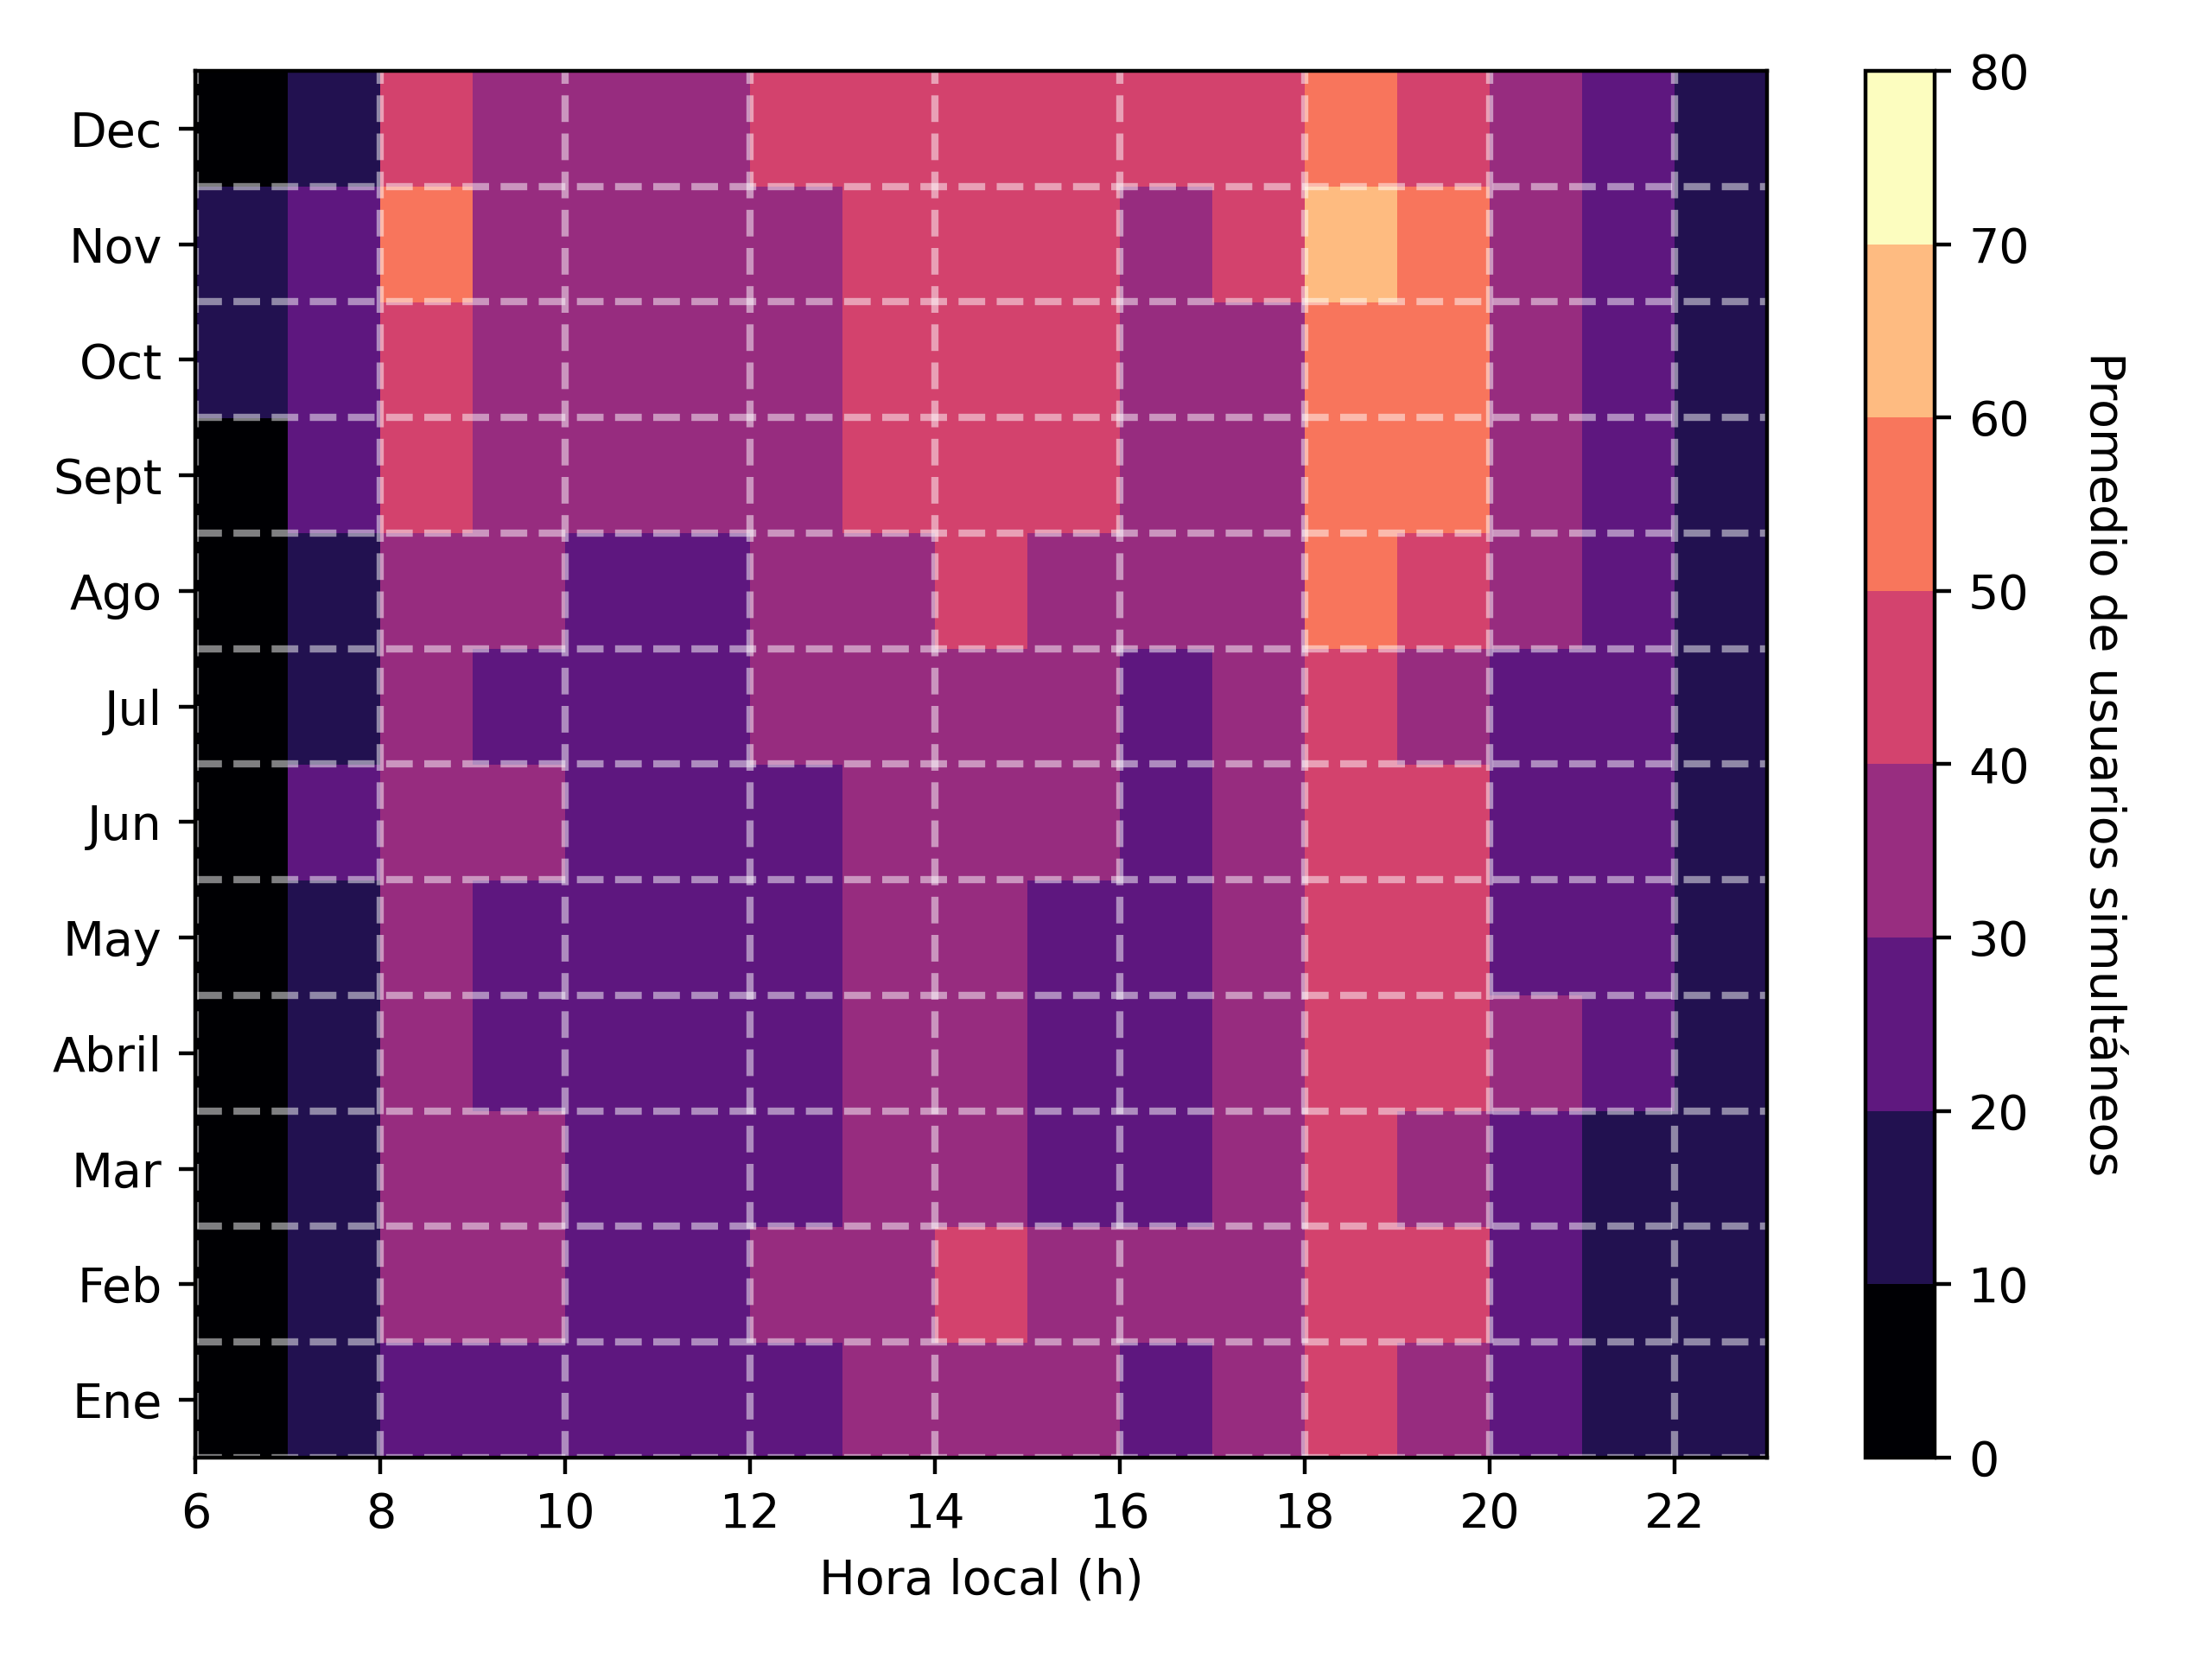
\includegraphics[width=8cm]{Graphics/monthly_hourly_mean_count_travel.png}
        \caption{Promedio mensual del número de usuarios.}
        \label{fig:monthly_hourly_mean_count_travel}
    \end{subfigure}
    \begin{subfigure}[b]{8cm}
        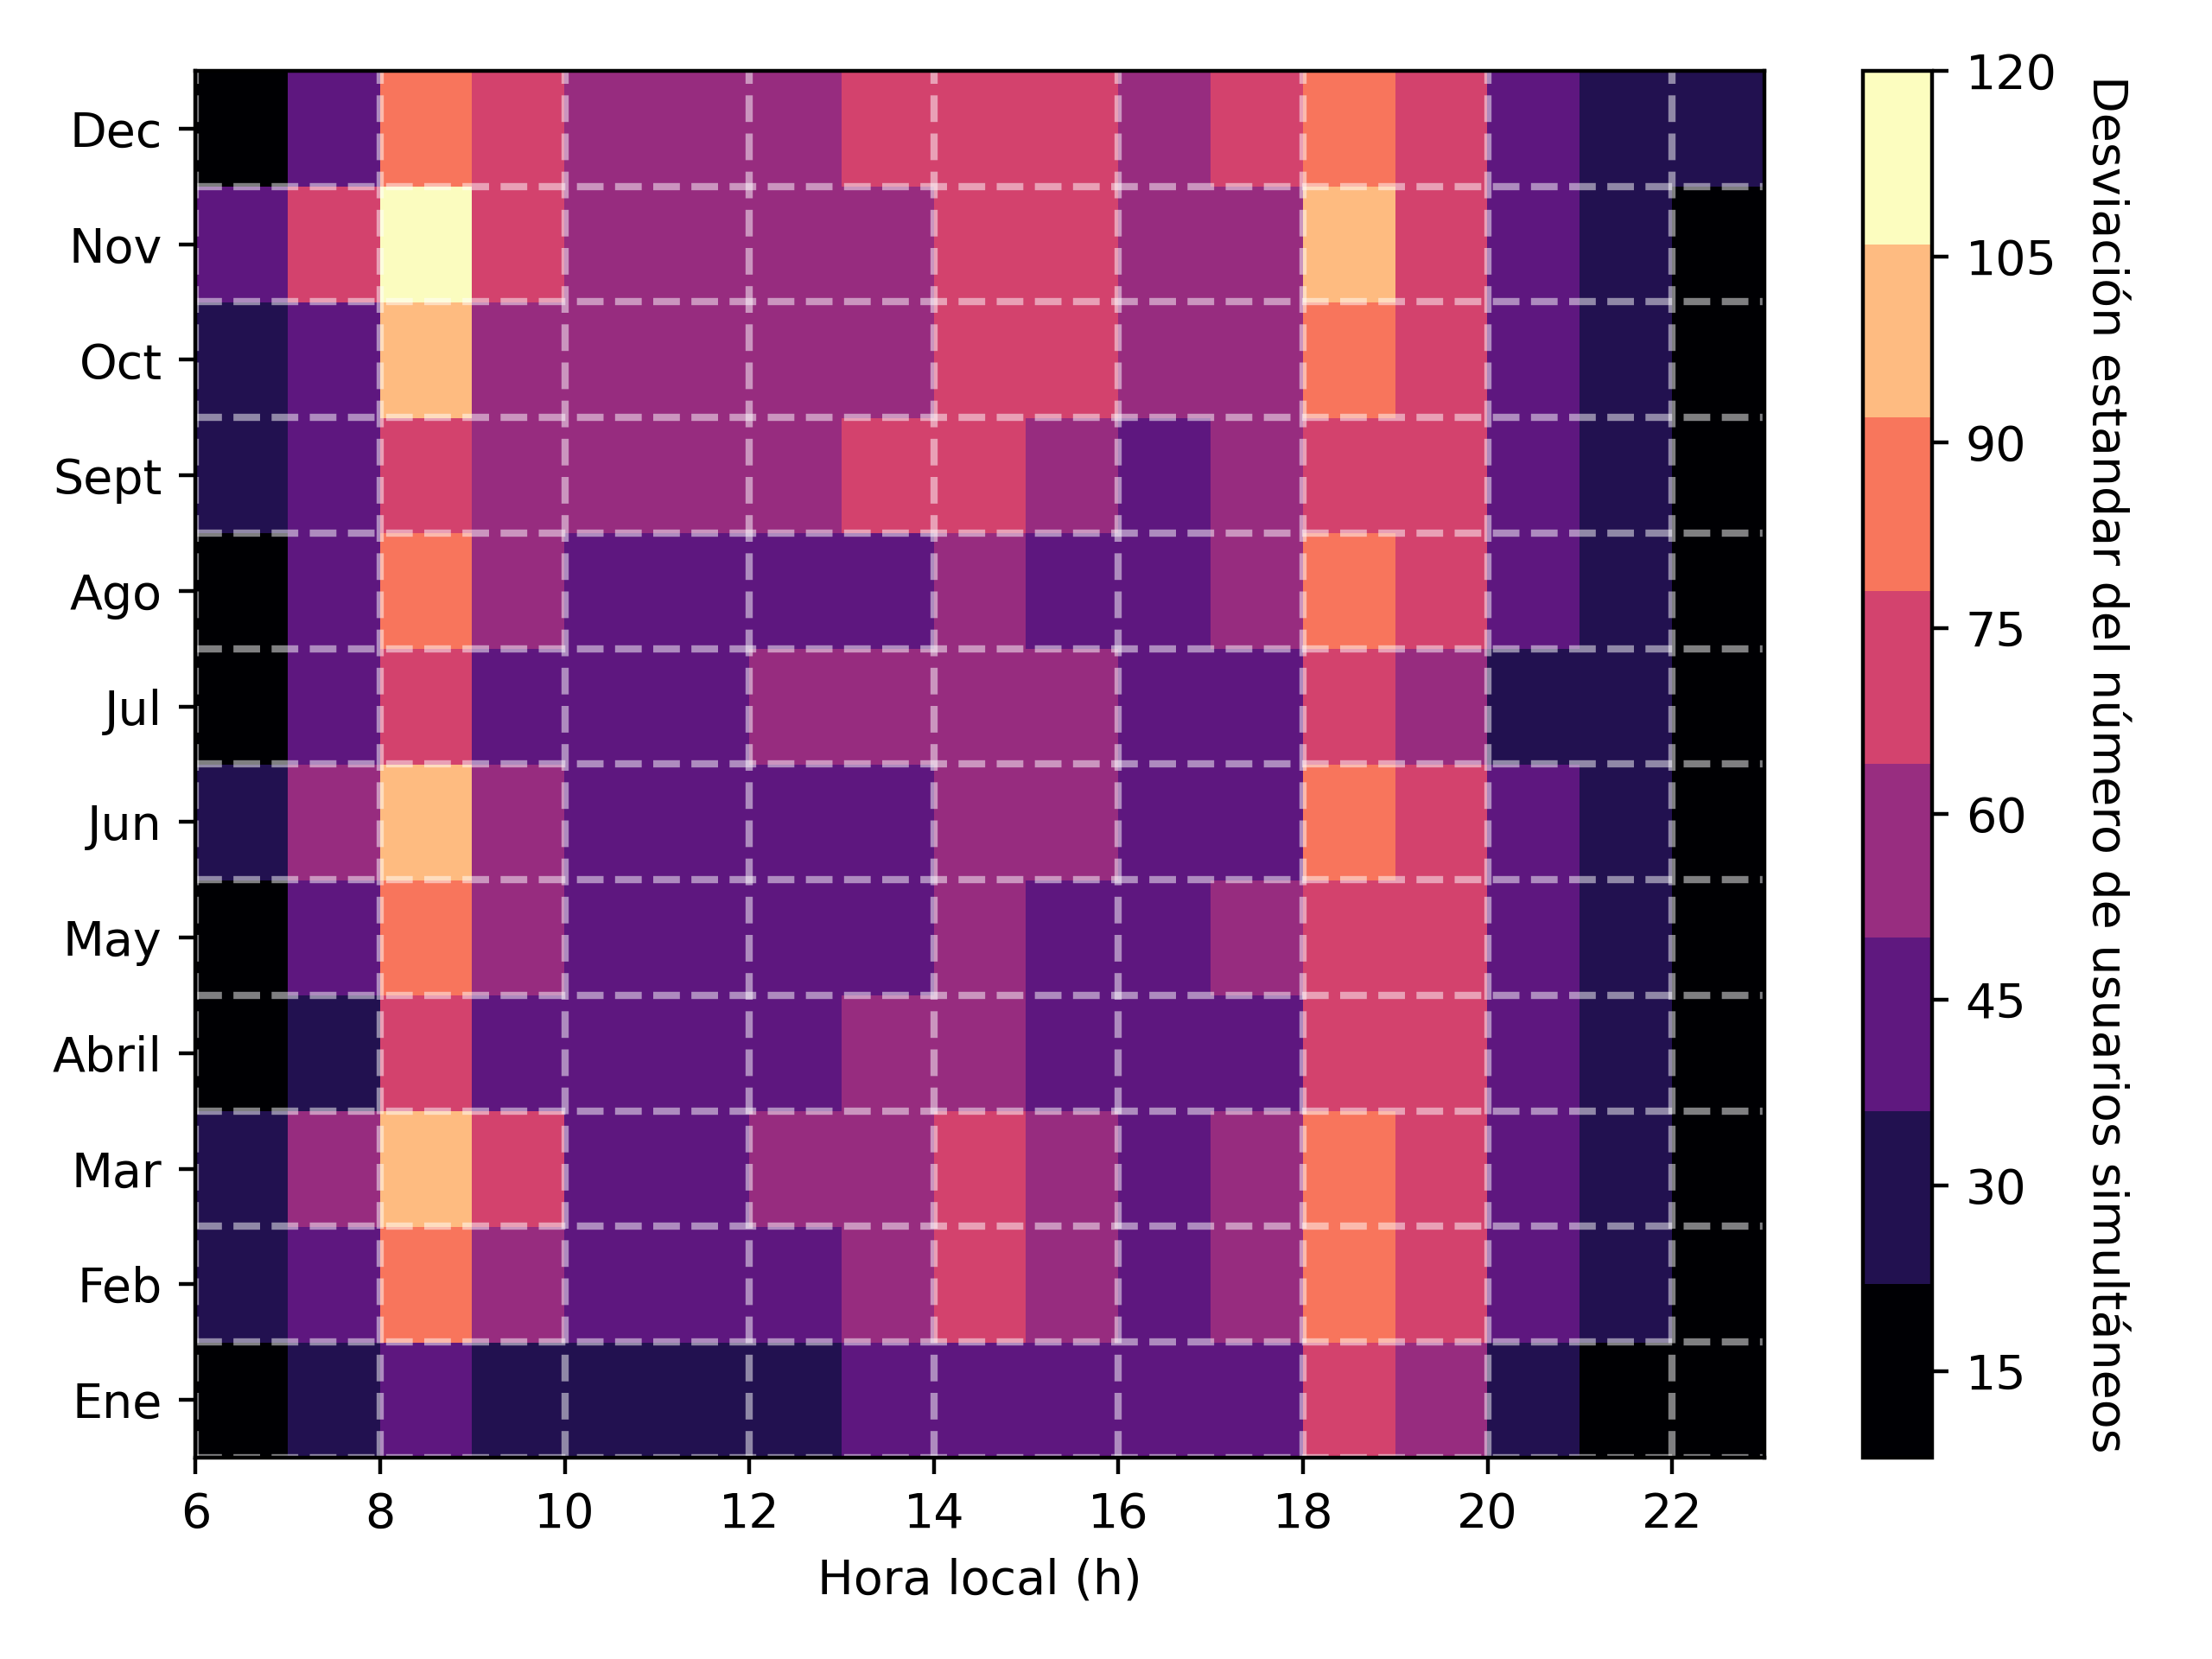
\includegraphics[width=8cm]{Graphics/monthly_hourly_var_count_travel.png}
        \caption{Desviación estandar del número de usuarios.}
        \label{fig:monthly_hourly_var_count_travel}
    \end{subfigure}
    \caption{Tiempo de uso promedio y desviación estandar mensual por hora de lo usuarios calculadas con las ecuaciones \ref{eq:monthly_hourly_mean_count_travel} y \ref{eq:monthly_hourly_var_count_travel}.}
    \label{fig:monthly_hourly_count_travel}
\end{figure}

\subsubsection{Promedios diarios semanales por hora}

Otra manera de abordar los datos es realizando un promedio del día semanal por las horas del día. Esto se obtuvo aplicando la ecuación \ref{eq:daily_hourly_mean_count_travel} a los datos.

\begin{equation}
    \bar{t}_{d,h} = \frac{1}{n_{(d,h)}} = \sum_{i=1}^{n_{(d,h)}} \hat{t}_{i} \qquad \begin{matrix}
        d=1,2,\dots,7 \\ h=6,7,\dots,23
    \end{matrix} \label{eq:daily_hourly_mean_count_travel}
\end{equation}

donde $V_i$ y $n_{(d,h)}$ es el conjunto y la cantidad total de viajes realizados para el día de la semana $d$ realizados entre las $h$ y $h+1$ horas respectivamente. De una manera semejante, se calculo la varianza de este conjunto con la ecuación \ref{eq:daily_hourly_var_count_travel}.

\begin{equation}
    \sigma_{V_{(d,h)}} = \frac{1}{n_{(d,h)}-1} \sum_{i=1}^{n_{(d,h)}} (V_i-\bar{V}_{(d,h)})^2 \qquad \begin{matrix}
        m=1,2,\dots,12 \\ h=6,7,\dots,23
    \end{matrix} \label{eq:daily_hourly_var_count_travel}
\end{equation}

En la figura \ref{fig:daily_hourly_count_travel} se muestran los resultados de aplicar las ecuaciones \ref{eq:daily_hourly_mean_count_travel} y \ref{eq:daily_hourly_var_count_travel} a los datos de las distancias.

En la figura \ref{fig:daily_hourly_mean_count_travel} se aprecia que existe una predilección en utilizar el servicio de bicicleta entre semana a las 8 y 16 horas. Existiendo un mínimo en el horario de 17 a 23 horas los días sabados y domingos. Con la figura \ref{fig:daily_hourly_var_count_travel} se observa que en el periodo donde existe un máximo, este presenta una gran variación, lo cual concuerda con lo encontrado en la figura \ref{fig:monthly_hourly_var_count_travel}. Por ende, se puede suponer que los usuarios que utilizan el servicio en ese periodo de tiempo pueden no ser recurrentes y usarlo cuando les sea necesario, más no es su primera opción.

\begin{figure}[H]
    \centering
    \begin{subfigure}[b]{8cm}
        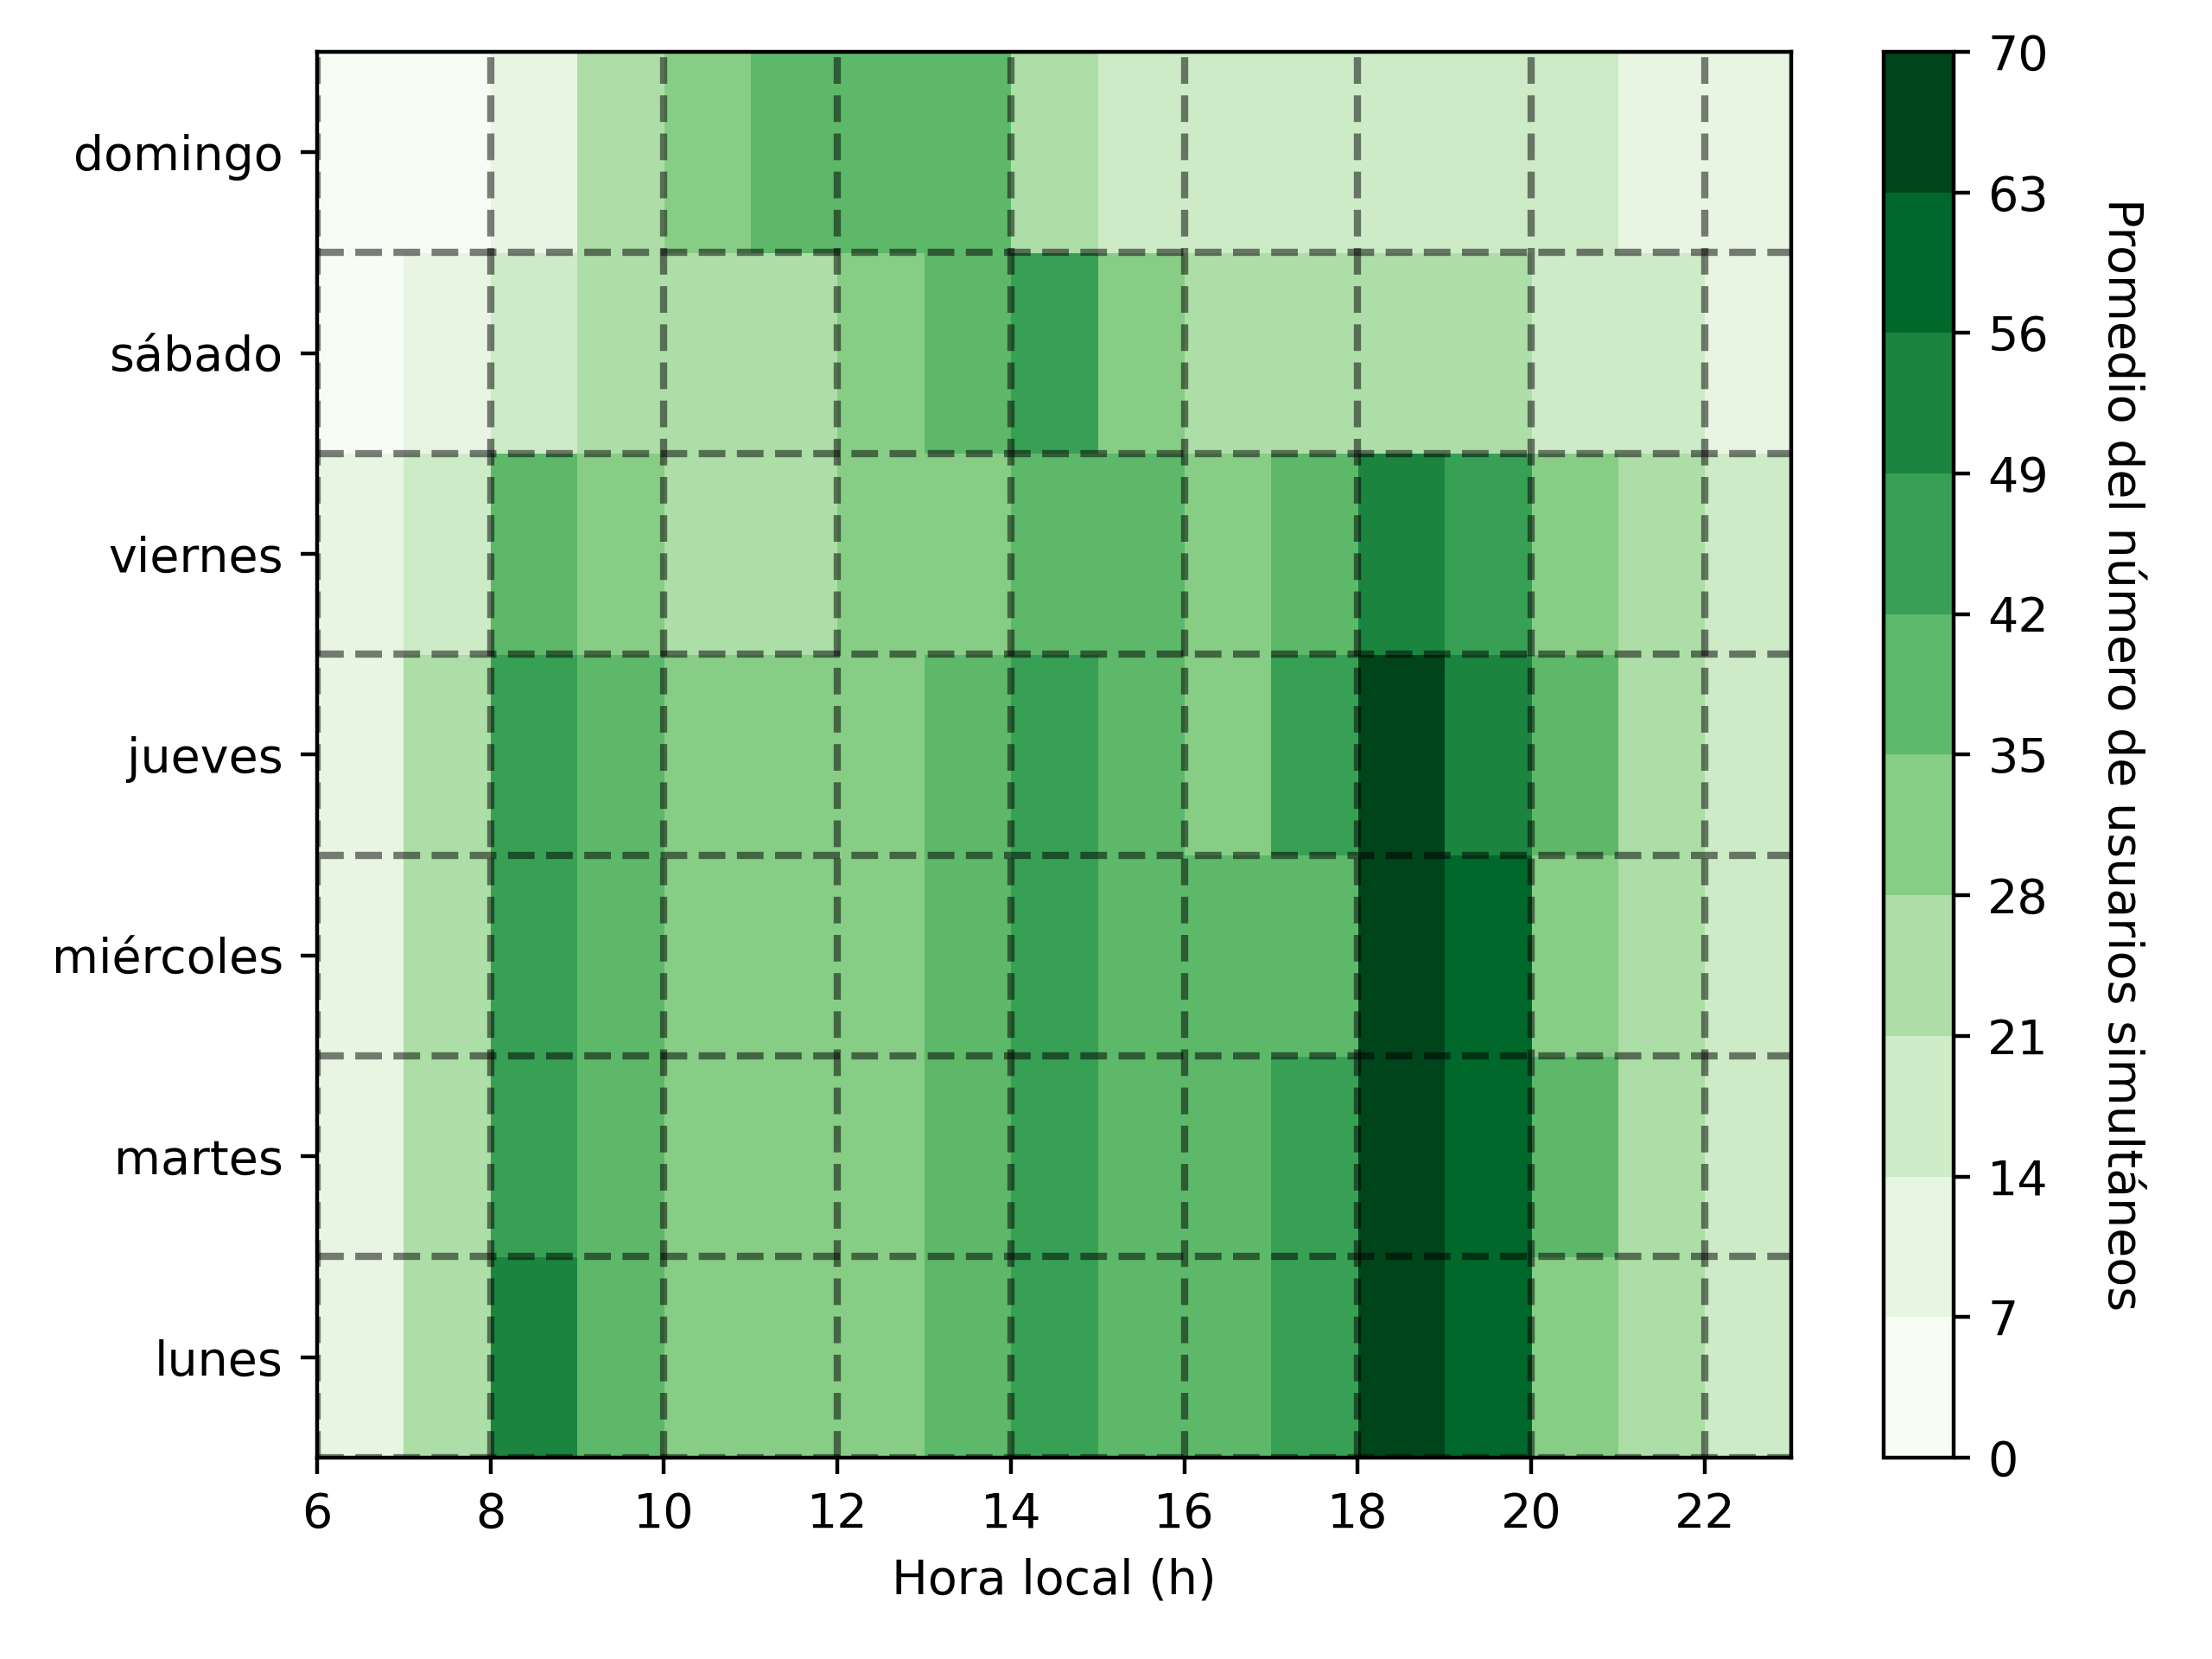
\includegraphics[width=8cm]{Graphics/daily_hourly_mean_count_travel.png}
        \caption{Promedio diaria del número de usuarios semanal.}
        \label{fig:daily_hourly_mean_count_travel}
    \end{subfigure}
    \begin{subfigure}[b]{8cm}
        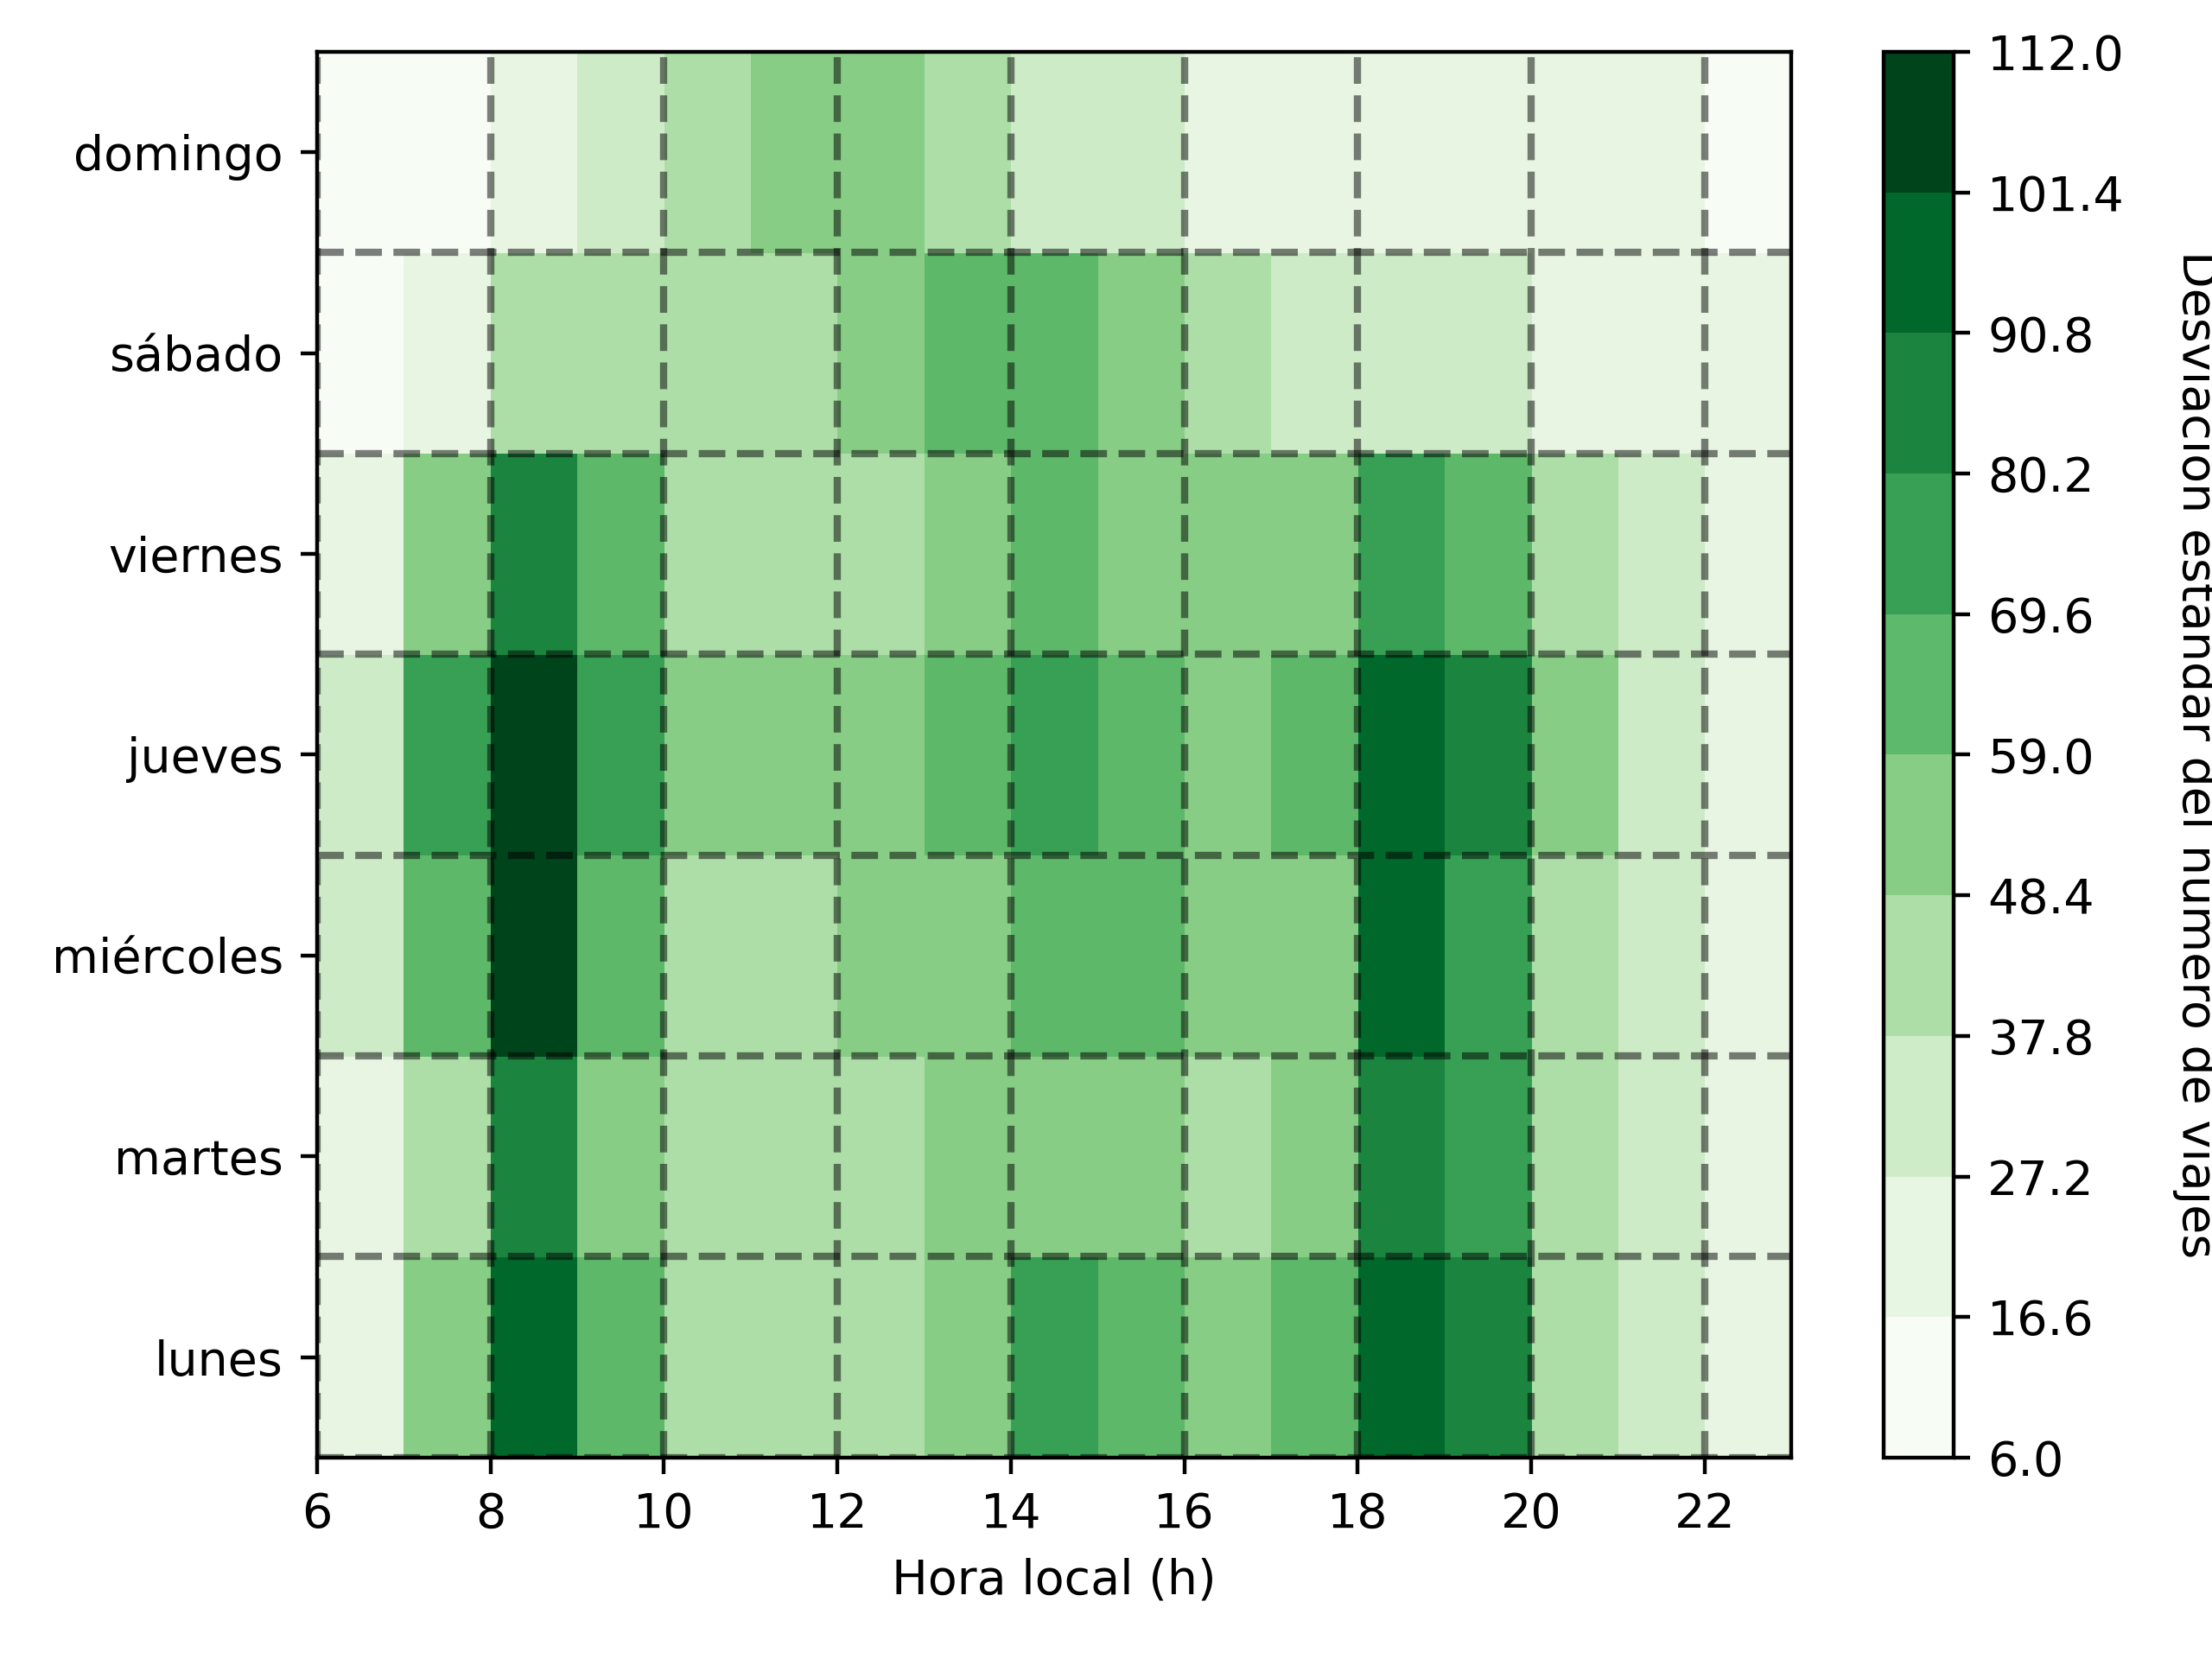
\includegraphics[width=8cm]{Graphics/daily_hourly_var_count_travel.png}
        \caption{Desviación estandar del número de usuarios semanal.}
        \label{fig:daily_hourly_var_count_travel}
    \end{subfigure}
    \caption{Número de usuarios promedio y desviación estandar diaria semanal por hora calculados con las ecuaciones \ref{eq:daily_hourly_mean_count_travel} y \ref{eq:daily_hourly_var_count_travel}.}
    \label{fig:daily_hourly_count_travel}
\end{figure}
